%# -*- coding:utf-8 -*-
\documentclass[10pt,aspectratio=169,mathserif]{beamer}		
%设置为 Beamer 文档类型,设置字体为 10pt,长宽比为16:9,数学字体为 serif 风格

%%%%-----导入宏包-----%%%%
\usepackage{zju}			%导入 zju 模板宏包
\usepackage{ctex}			%导入 ctex 宏包,添加中文支持
\usepackage{amsmath,amsfonts,amssymb,bm}   %导入数学公式所需宏包
\usepackage{color}			 %字体颜色支持
\usepackage{graphicx,hyperref,url}
\usepackage{metalogo}	% 非必须
%% 上文引用的包可按实际情况自行增删
%%%%%%%%%%%%%%%%%%
\usepackage{fontspec}
\usepackage{xeCJK}
\usepackage{subfigure}
\usepackage{palatino}
% \setCJKmainfont{Source Han Sans SC}
% \setsansfont{Arial}

\renewcommand{\figurename}{Fig}

\beamertemplateballitem		%设置 Beamer 主题

%%%%------------------------%%%%%
\catcode`\。=\active         %或者=13
\newcommand{。}{.}				
%将正文中的“。”号转换为“.”。中文标点国家规范建议科技文献中的句号用圆点替代"latex-workshop.latex.autoBuild.run": "onFileChange",
%%%%%%%%%%%%%%%%%%%%%

%%%%----首页信息设置----%%%%
\title[短期科学研究探索]{
  短期科学研究探索}
\subtitle{阶段一报告}			
%%%%----标题设置


\author[韩耀霆]{
  HAN YAOTING \\\medskip
  {\small \url{3220101611@zju.edu.cn}} \\
  {\small 数学科学学院}}
% \author[HAN YAOTING]{
%   HAN YAOTING \\\medskip
%   % {\small \url{3220101611@zju.edu.cn}} \\
%   {\small AI4Math}}
%%%%----个人信息设置
  
\institute[IOPP]{
  脑机接口国家重点实验室}
% \institute[IOPP]{
%   State Key Laboratory of Computer Aided Design and Graphics (CAD\&CG)\\ 
%   Zhejiang University}
%%%%----机构信息

\date[\today]{
  \today}
%%%%----日期信息
  
\begin{document}

\begin{frame}
	\titlepage
\end{frame}				%生成标题页

\section{目录}
\begin{frame}
	\frametitle{目录}
	\tableofcontents
\end{frame}				%生成提纲页

\section{内容简介}
\begin{frame}
	\frametitle{主要内容}

    \begin{itemize}
      \item SNN的相关基本概念
      \item 了解熟悉SNN中的一种神经元、架构、编解码和学习策略
      \item 搭建一个简单的SNN网络完成对MNIST的训练和评估
      \item 粗略阅读一篇前沿文章
    \end{itemize}
        
\end{frame}

\begin{frame}
	\frametitle{整体思路}

    \begin{itemize}
      \item 了解SNN的基本情况
      \item 通过综述文章了解SNN的相关研究进展(神经元模型、架构等)
      \item 通过snnTorch对每个版块熟悉一种结构
      \item 使用PyTorch框架自己实现一个SNN网络并完成一个简单的任务
      \item 阅读一篇前沿文章,了解SNN的最新研究进展
    \end{itemize}
        
\end{frame}

\section{SNN的基本情况}
\begin{frame}
	\frametitle{SNN简介}

    \begin{columns}

    \column{0.55\textwidth}
        \begin{itemize}
            \item SNN将ANN中的“仿射变化+激活函数”的人工神经元替换为了生物合理性更强的“微分方程刻画的膜电位变化+脉冲触发”的类生物神经元。
            \item SNN是为了更好地模拟生物大脑中的神经元传递信息的方式,使之相比ANN更加高效节能,且在生物角度上更加合理。
        \end{itemize}

    \column{0.45\textwidth}
    \begin{figure}
        \centering
        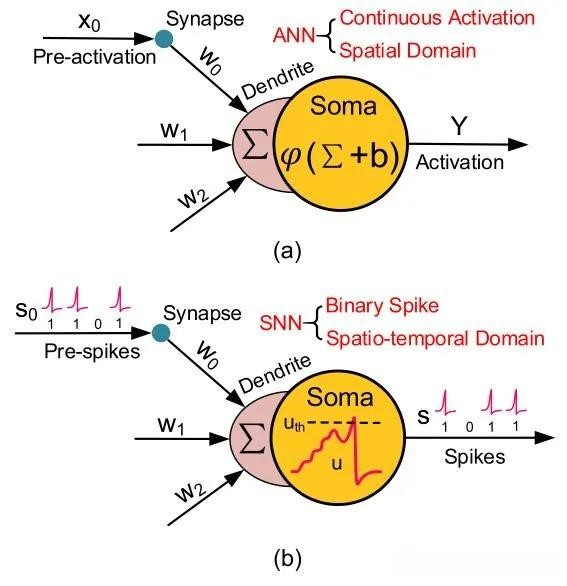
\includegraphics[width=0.85\linewidth]{figures/ANN_SNN.jpg}
    \end{figure}
    \end{columns}
        
\end{frame}

\begin{frame}
	\frametitle{SNN的结构简述}

    \begin{itemize}
        \item \textbf{信息编码}:常见的编码方式分为速率编码和时间编码两种。
        \item \textbf{神经元}:SNN中最基本的结构,基于类R-C电路微分方程给出神经元膜电位变化,在膜电位达到阈值后触发一个脉冲。
        \item \textbf{神经回路}:连接若干神经元的网络,它一定是一个前馈网络,但可以通过加入前/反/侧馈抑制来实现更多的功能。
        \item \textbf{学习策略}:一般有ANN2SNN的间接训练和有/无监督直接训练两种大的策略。
    \end{itemize}
        
\end{frame}

\begin{frame}
	\frametitle{信息编码}

        \begin{itemize}
            \item \textbf{速率编码}:基于脉冲发放频率来表示信息,脉冲发放频率与像素强度成正比,常见的有计数/密度/群体频率编码,例如,计数频率编码的表示如下:
                $$ v = \frac{N_{spike}}{T} $$
                
            \item \textbf{时间编码}:通过神经元接收到输入刺激后首次发放脉冲的时间来量化输入刺激的强度,常见的有首达时间/排名顺序/相位编码,例如,首达时间编码的表示如下:
                $$t_{\text{spike}} = \min\{t \geq 0 \mid V(t) \geq V_{\text{thresh}}\}$$
            \item 两种编码理论上是在大脑中协同工作的,速率编码倾向于刻画长时持续的刺激行为,时间编码倾向于刻画单次发生的刺激行为。
        \end{itemize}
        
\end{frame}

\begin{frame}
	\frametitle{简化的Leaky Integrate-and-Fire(LIF)神经元}
        
        常用的神经元模型,它假设神经元的膜电位是由一个积分器和一个漏电导组成的,当膜电位超过一定的阈值时,神经元会被激发,并产生一个动作电位。然后,膜电位会被重置并进入不应期。其数学定义如下:
            $$C\frac{dV}{dt} = -g_L(V(t) - E_L) + I(t) $$
        如果我们取膜时间常数 $\tau = RC$,则上式变为
            $$\tau \frac{dV_{mem}}{dt} = -[V_{mem}(t) - V_{rest}] + RI(t) $$
        上述模型经过简化和向前欧拉方法后得到
            $$U(t + \Delta t) = \left(1 - \frac{\Delta t}{\tau}\right)U(t) + \frac{\Delta t}{\tau}I_{\text{in}}(t)R$$
        同时在触发后膜电位会重置,结合后得到表达式:
            $$U[t + 1] = \underbrace{\beta U[t]}_{\text{decay}} + \underbrace{W X[t+1]}_{\text{input}} - \underbrace{S[t] U_{\text{thr}}}_{\text{reset}}$$
\end{frame}

\begin{frame}
	\frametitle{神经回路}
        
        \begin{itemize}
            \item \textbf{前馈兴奋}:如图A,在每一层中,每个神经元通过汇聚连接从多个前突触节点接收输入,并自身发散连接到多个后突触等效物。
            \item \textbf{前馈/反馈抑制}:如图B,FB抑制指的是一层前突触兴奋性神经元会刺激投射回前突触兴奋性层的后突触兴奋性神经元以及抑制性神经元,反过来,FF抑制指的是后突触抑制性神经元群体连接到后突触神经元群体的情况。
            \item \textbf{侧抑制}:如图C,包括一些神经元呈现以减少并行通路活动的容量。通过这种方式,可以在减少传输不太相关脉冲的同时激发某些活动。
        \end{itemize}

        \begin{figure}
            \centering
            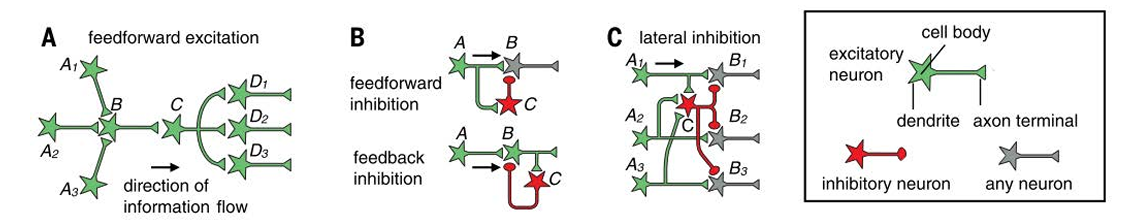
\includegraphics[width=0.75\linewidth]{figures/Neural_circuits.png}
        \end{figure}
        
\end{frame}

\begin{frame}
	\frametitle{替代梯度法的BP策略}
        
        这里我们考虑有监督学习的直接训练方法,ANN中的常见学习算法是对损失函数做关于参数矩阵的进行梯度下降以最小化损失函数,通过BP更新网络中的权重,但对LIF神经元,由链式法则得到
            $$\frac{\partial L}{\partial W} = \frac{\partial L}{\partial S} \underbrace{\frac{\partial S}{\partial U}}_{\{0,\infty\}} \frac{\partial U}{\partial I} \frac{\partial I}{\partial W}$$
        其中$S$和$U$之间关系由下Heaviside 阶跃函数替代
            $$S[t] = \Theta(U[t] - U_{\text{thr}})$$
        它的导数是狄拉克函数,显然在定义域上非0即无穷,无法直接进行学习,一种可行的解决方案是在FP时保持 Heaviside 函数的不变,在BP时使用它的平滑函数去拟合导数结果,常用的函数是正反切函数,其导数如下:
            $$\frac{\partial \tilde{S}}{\partial \bar{U}} \leftarrow \frac{1}{\pi} \frac{1}{(1 + (U \pi)^2)}$$
        这就使得BP时的导数计算成为可能。
        
\end{frame}

\section{SNN的手写数字分类}
\begin{frame}
	\frametitle{SNN结构简介}

        一个3层全连接SNN,每层神经元数量为784、1000、10,使用归一化静态MNIST特征作为输入进行类速率编解码,简化的LIF神经元,前馈兴奋神经回路,替代梯度的反向传播有监督学习策略,网络结构大致如下:

        \begin{figure}
            \centering
            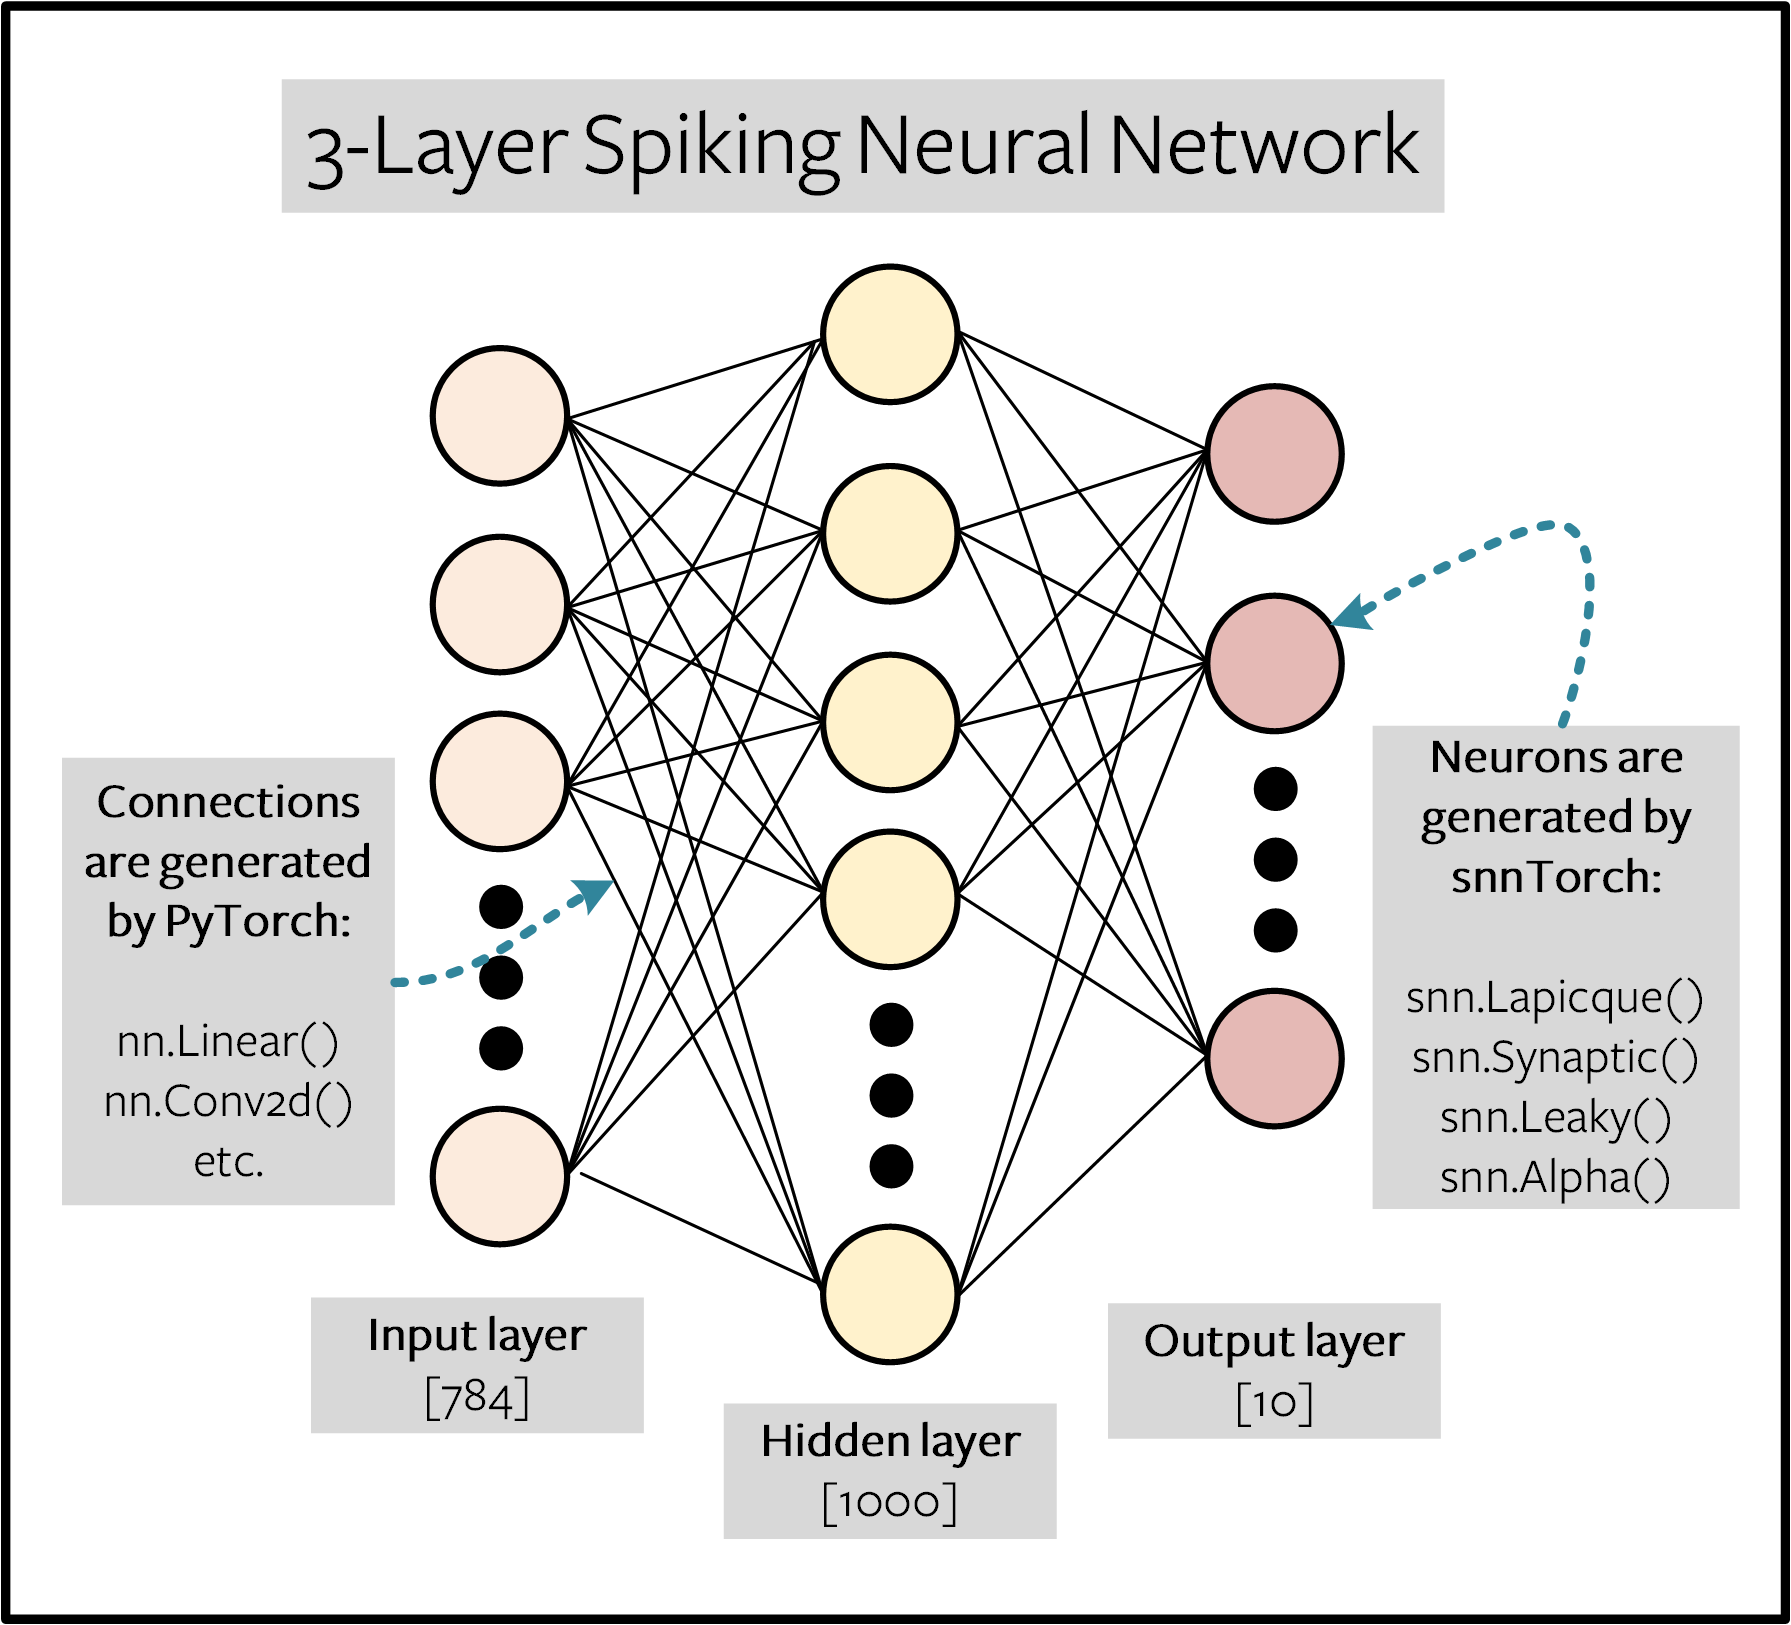
\includegraphics[width=0.4\linewidth]{figures/MNIST_3LaySNN.png}
        \end{figure}
        
\end{frame}

\begin{frame}
	\frametitle{训练结果}

        参考snnTorch用户手册,在copilot辅助下使用snnTorch框架和PyTorch框架分别搭建上述网络,在A800上用5个epoch训练得到结果如下:

        \begin{figure}
            \centering
            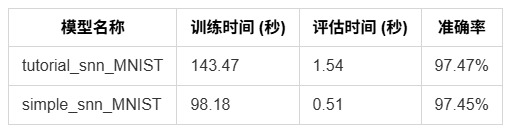
\includegraphics[width=0.6\linewidth]{figures/MNIST_Result.png}
        \end{figure}

        在基础配置完全相同的情况(归一化策略、epoch数量等)下,二者的表现接近,训练与评估时间上的差别是由于代码实现不同(初始化方法、加速与否等)导致的。

        额外地,simple\_snn\_MNIST 的 forward 只返回最后一层的脉冲均值,其损失计算并不在每个时间步计算累加。

\end{frame}

\begin{frame}
	\frametitle{Loss曲线}

        我们对训练过程中的Loss曲线绘制如下:

        \begin{columns}
        
            \column{0.5\textwidth}
            
            \begin{figure}
                \centering
                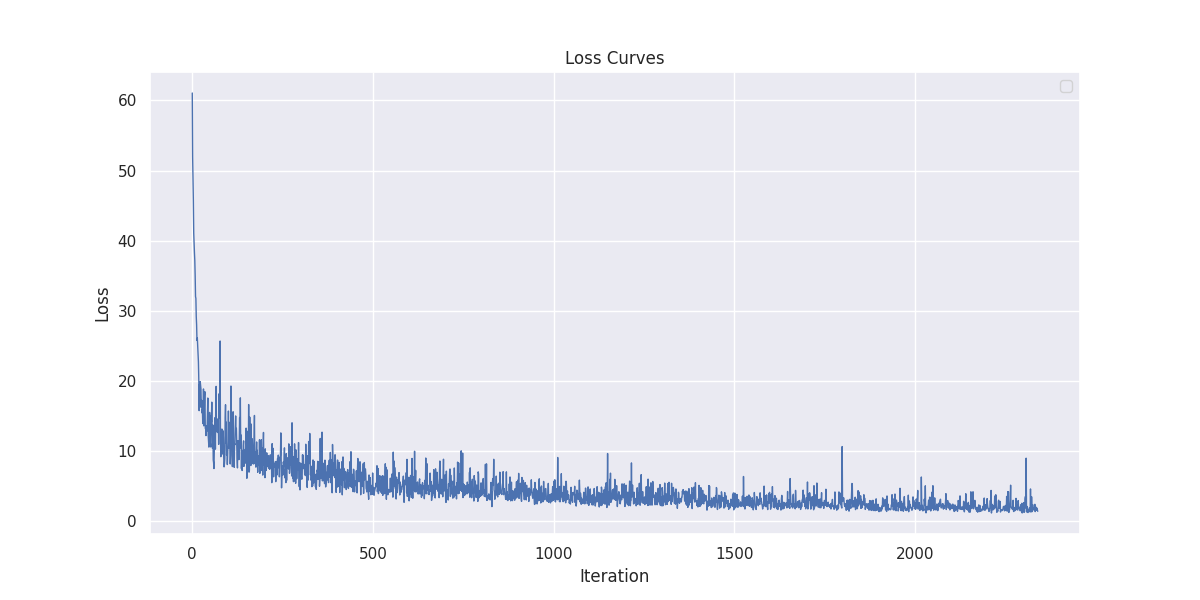
\includegraphics[width=1.1\linewidth]{figures/tutorial_snn_MNIST_Loss.png}
                \caption{snnTorch搭建网络损失函数}
            \end{figure}

            \column{0.5\textwidth}

            \begin{figure}
                \centering
                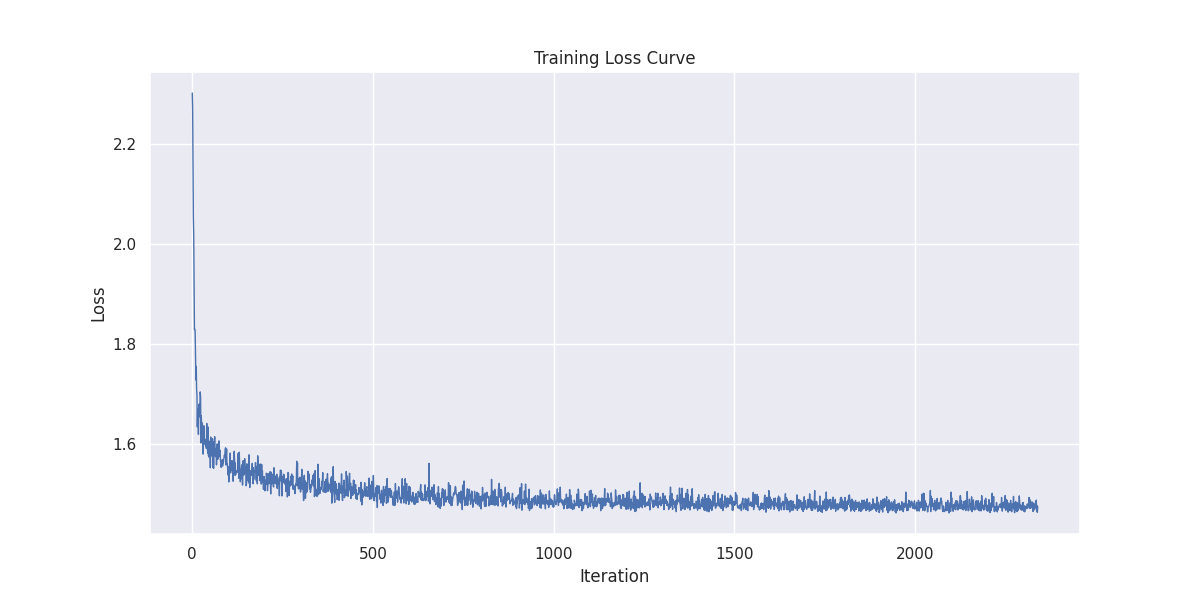
\includegraphics[width=1.1\linewidth]{figures/simple_snn_MNIST_Loss.png}
                \caption{PyTorch搭建网络损失函数}
            \end{figure}
 
        \end{columns}

        二者在误差允许范围内是相似的且下降速度符合预期。

\end{frame}

\begin{frame}
	\frametitle{改进空间}

    \begin{itemize}
        \item 网络对MNIST针对性极强,需要进一步调整网络层数、宽度和数据输入策略。
        \item 本质上这只是将ANN中的神经元和学习策略做了替换得到的,生物合理性不高,需要进一步调整数据的编解码方式。
        \item 完善SNN的相关功能,扩展神经元类型、学习策略等。
    \end{itemize}

\end{frame}

\section{附录}
\begin{frame}
	\frametitle{附录}

    \begin{itemize}
        \item \textbf{源文件}:
        
            存储在github项目\url{https://github.com/DrypotTofu/BMI_project}中。
        \item \textbf{清单}:
            \begin{itemize}
                \item Transformer?
                \item 混合编码形式?
                \item ANN2SNN的转化过程?STBP?TDBN?FT?
                \item 神经元连接的可生长性?
            \end{itemize}
        
    \end{itemize}
    

\end{frame}

\section{参考资料}
\begin{frame}
  \frametitle{参考资料}
	  \begin{thebibliography}{99}
      \bibitem{bilibili_snn} 脉冲神经网络(SNN)概览, {\sl 脉冲神经网络概览}, 2023, \url{https://www.bilibili.com/video/BV1dG4y1D7b2/}

      \bibitem{nunes2022} João~D.~Nunes, Marcelo~Carvalho, Diogo~Carneiro, and Jaime~S.~Cardoso, {\sl Spiking Neural Networks: A Survey}, 2022

      \bibitem{eshraghian2023} Jason~K.~Eshraghian, Max~Ward, Emre~O.~Neftci, Xinxin~Wang, Gregor~Lenz, Girish~Dwivedi, Mohammed~Bennamoun, Doo~Seok~Jeong, and Wei~D.~Lu, {\sl Training Spiking Neural Networks Using Lessons From Deep Learning}, 2023

      \bibitem{xu2025} Mengting~Xu, De~Ma, Huajin~Tang, Qian~Zheng, and Gang~Pan, {\sl FEEL-SNN: robust spiking neural networks with frequency encoding and evolutionary leak factor}., 2025
	  \end{thebibliography}

\end{frame}

\end{document}